\chapter{Analysis of the Impact of Heterogeneity Losses due to Upscaling in Well Testing Simulations}

Chapters \ref{mathematicalFormulation} to \ref{solution} show how the reservoir simulator utilized in this project has been developed and validated. Chapters \ref{upscaling} and \ref{wellTesting} show introductions of upscaling and well testing, the areas of application of the simulator developed in this project. This chapter show the main utilization of this simulator in this project: analyzing the effects of upscaling in well testing simulations. Several models have been created and put under flow simulation. The results of bottom hole pressure, pressure drop and Bourdet derivative have been plot and compared. The first section of this chapter shows the details of each of those models and the parameters of the simulation. Then, the last section will show the results obtained in the simulation and its analyzes.

\section{Models}

Eight different cases have been created and simulated for outputing bottom hole pressure, pressure drop, and the Bourdet derivative. They are parallelepipedal models of synthetic sandstone reservoirs. Table \ref{table10.1} shows the characteristics that are common for all the cases. The fluid model for all the scenarios is the same as utilized in the validation cases and is illustrated by Figure \ref{fig:30}. The porosity-permeability relationship is equal for all the models and follows the correlation illustrated in Figure \ref{fig:35} and in the Eq. \ref{results1}.
\begin{table}[htbp]
	\centering
	\caption{Common characteristics for all the simulation cases.}
	\begin{tabular}{c c}
	\toprule
	Parameter & Value (if applicable)\\
	\midrule
	Reservoir length in the $x$ direction & 2559.03 ft\\
	Reservoir length in the $y$ direction & 2559.03 ft\\
	Reservoir length in the $z$ direction & 164.04 ft\\
	Sealed reservoir: no flow in the boundaries\\
	Vertical well in the center of the reservoir\\
	Completions from the top to the bottom of the reservoir\\
	Average porosity & 20\%\\
	Average horizontal permeability & 51.59 mD\\
	Average vertical permeability & 51.59 mD\\
	Formation compressibility & $1.31 x 10^{-4}$ psi$^{-1}$\\
	Fluid compressibility &  1.41 x 10$^{-5}$ psi$^{-1}$\\
	Depth of the topmost layer & 10,498.69 ft\\
	Reference depth for the initial pressure & 10,498.69 ft\\
	Initial pressure at the reference depth & 3,916.01 psi\\
	Well radius & 6 in\\
	Skin factor & -0.5\\
	\bottomrule
\end{tabular}
	\label{table10.1}
\end{table}

\begin{figure}[H]
	\centering
	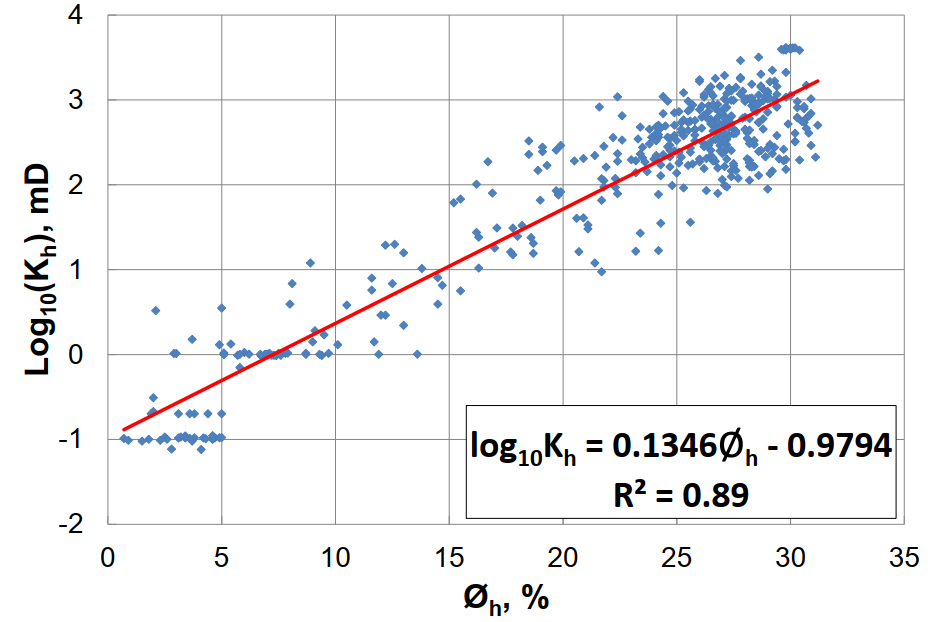
\includegraphics[width=0.8\linewidth]{Images/35}
	\caption{Correlation between porosity and permeability for all the simulated scenarios. This relationship is the same as the UNISIM-I model, a synthetic sandstone model based in the Namorado Field, Campos Basin of Brazil. Source: \cite{Avansi2015}}
	\label{fig:35}
\end{figure}

\begin{equation}\label{results1}
k_h = 10^{(0.1346\phi)-0.9794}.
\end{equation}

What differs one case to another is the size and number of the grid blocks and the standard deviation of the porosity and permeability. Table \ref{fig:36} shows a table describing the characteristics of each scenario.

\begin{table}[htbp]
	\centering
	\caption{Diference between each simulation scenario.}
	\label{fig:36}
	\begin{tabular}{c c c c c c c}
		\toprule
		Case & Nx & Ny & Nz & Upscaling & Heterogeneity & $\phi$ Standard Deviation\\
		\midrule
		1 & 26 & 26 & 20 & No & Homogeneous & 0\\
		2 & 13 & 13 & 10 & No & Homogeneous & 0\\
		3 & 26 & 26 & 20 & Yes & Heterogeneous & 3\%\\
		4 & 13 & 13 & 10 & Yes & Heterogeneous & 6\%\\
		5 & 26 & 26 & 20 & Yes & Heterogeneous & 6\%\\
		6 & 13 & 13 & 10 & Yes & Heterogeneous & 6\%\\
		7 & 26 & 26 & 20 & Yes & Heterogeneous & 1.5\%\\
		8 & 13 & 13 & 10 & Yes & Heterogeneous & 1.5\%\\
		\bottomrule
	\end{tabular}
\end{table}

%\begin{figure}[H]
%	\centering
%	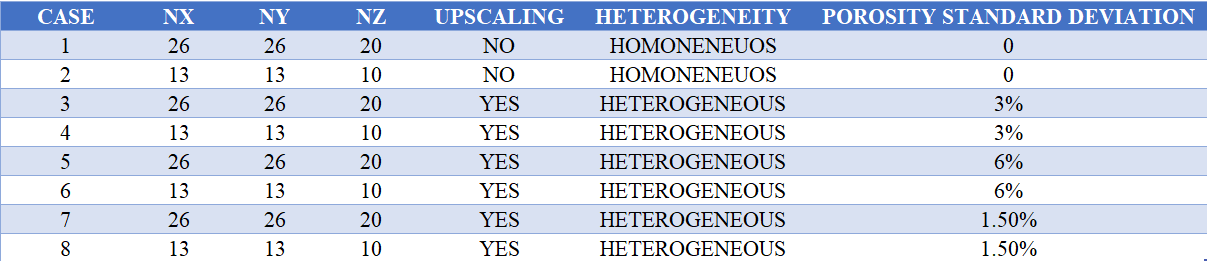
\includegraphics[width=1\linewidth]{Images/36}
%	\caption{Difference between each simulation scenario.}
%	\label{fig:36}
%\end{figure}

Scenario 1 is a fine homogeneous reservoir, scenario 2 is the same reservoir but coarsened, each direction of scenario 2 presents half the number of grid blocks in comparison to scenario 1. This scaling up has been done straightforwardly, the case is homogeneous and an averaging technique is not necessary. 

Scenario 3 is similar to scenario 1 but with heterogeneous permeabilities and porosities. The porosity follows a normal distribution with mean  20\%, the same as the one of scenario 1, and a standard deviation of 3\%. The horizontal permeability has been distributed by utilizing the correlation presented in Figure \ref{fig:31} and in the Eq. \ref{results1}. Furthermore, the vertical permeability has been set to be 10\% the value of the horizontal for each cell. Thus, both the vertical and horizontal permeabilities follow a log-normal distribution of means equal to the ones of scenario 1. Scenario 4 is the coarsened version of scenario 3. An arithmetic-harmonic averaging technique has been utilized for scaling up the permeability tensor as shown in the Eq. \ref{arithmeticharmonic}. For upscaling the porosity, a simple volumetric averaging technique has been utilized, as seen in the Eq. \ref{Upscaling3}. The Figures \ref{fig:37} to \ref{fig:39} show the porosity and permeability distributions for both the case 3 and case 4.

\begin{figure}[H]
	\centering
	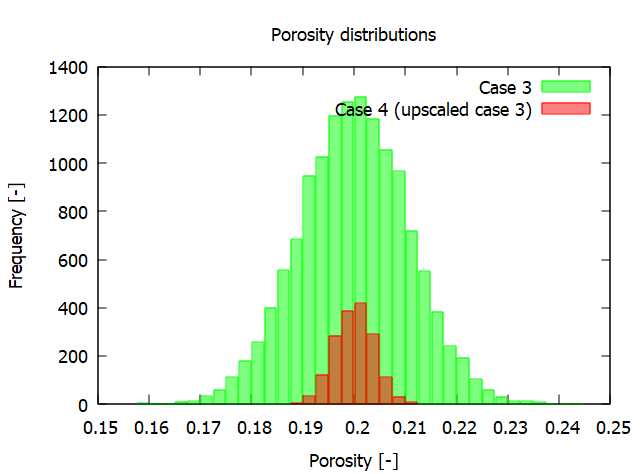
\includegraphics[width=0.8\linewidth]{Images/37}
	\caption{Porosity distribution for case 3 and its upscaled version (case 4).}
	\label{fig:37}
\end{figure}

\begin{figure}[H]
	\centering
	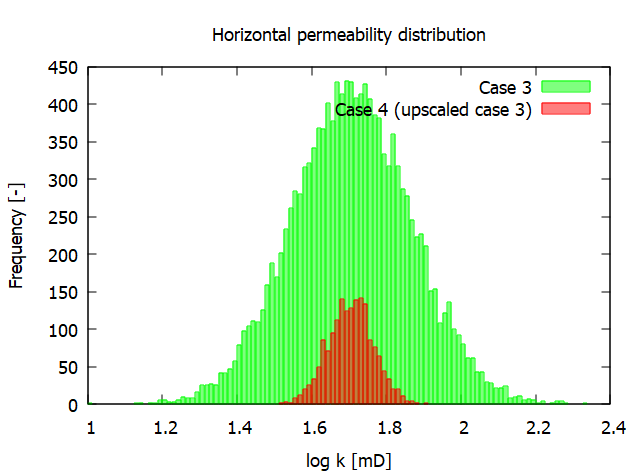
\includegraphics[width=0.8\linewidth]{Images/38}
	\caption{Horizontal permeability distribution for case 3 and its upscaled version (case 4).}
	\label{fig:38}
\end{figure}

\begin{figure}[H]
	\centering
	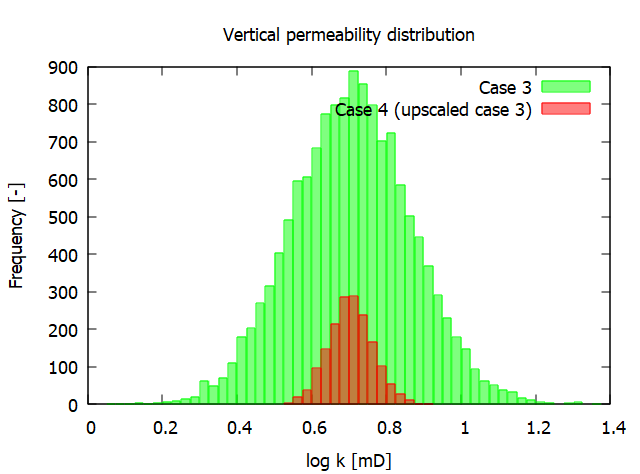
\includegraphics[width=0.8\linewidth]{Images/39}
	\caption{Vertical permeability distribution for case 3 and its upscaled version (case 4).}
	\label{fig:39}
\end{figure}

Figures \ref{fig:37} to \ref{fig:39} display the petrophysical distributions for both the fine grid and its upscaled model. One could see that the red histograms' columns (upscaled model) are smaller than the green ones (fine model), that happens because the number of grid blocks for the coarse model is eight times less than in the fine one. Since the vertical axis displays the frequency in absolute terms, the upscaled model has naturally smaller columns. Another difference between the red and green is the dispersion: the standard deviation of the fine model is superior to the one of the upscaled version. That is a natural characteristic of the upscaling: the grid blocks were averaged implying in a lower dispersion in the coarse model. Figures \ref{fig:42} to \ref{fig:44} show the distribution of the other cases.

All those cases have been put under flow simulations for a drawdown test scenario, in which the well is set to be initially closed and opens at the time 0.1 day, with the simulation ending at the time of 2 days. Figures \ref{fig:47} to \ref{fig:48} display the outputs of bottom hole pressure for the simulations. Figures \ref{fig:51} to \ref{fig:55} shows the log-log diagnostic plot for this drawdown test, comprising the pressure drop and Bourdet derivative curves for each case. 

Figure \ref{fig:46} shows the BHP for all the fine models. One could see that the results for the homogeneous model (case 1) were very similar to the ones of the model with a lower standard deviation (case 7). The BHP for case 5 (higher standard deviation) was considerably higher than the ones for the cases with lower dispersions.

\begin{figure}[H]
	\centering
	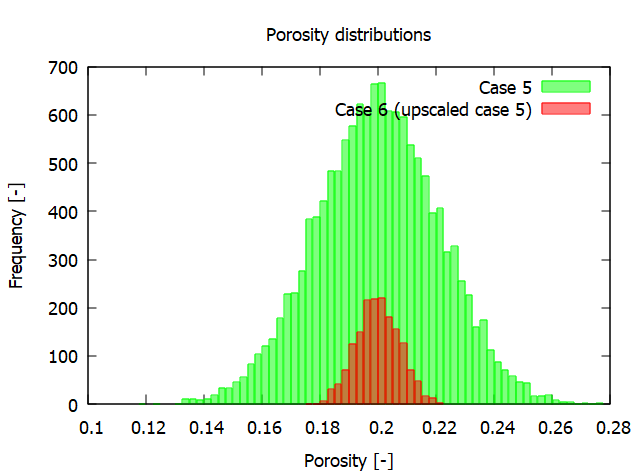
\includegraphics[width=0.8\linewidth]{Images/42}
	\caption{Porosity distribution for case 5 and its upscaled version (case 6).}
	\label{fig:42}
\end{figure}

\begin{figure}[H]
	\centering
	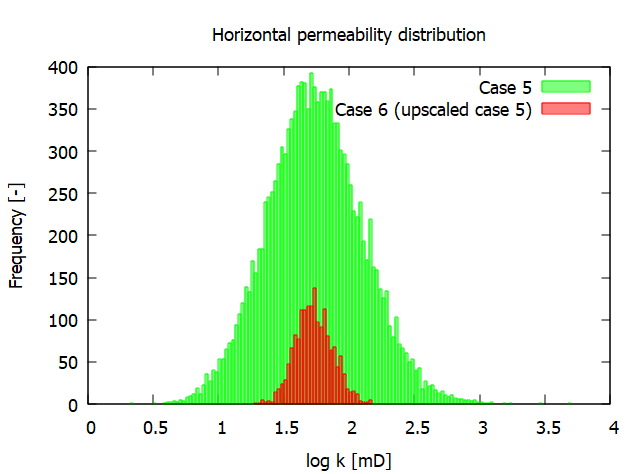
\includegraphics[width=0.8\linewidth]{Images/41}
	\caption{Horizontal permeability distribution for case 5 and its upscaled version (case 6).}
	\label{fig:41}
\end{figure}

\begin{figure}[H]
	\centering
	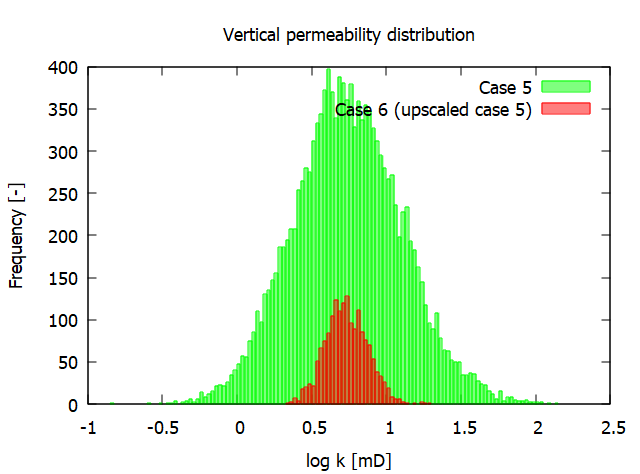
\includegraphics[width=0.8\linewidth]{Images/40}
	\caption{Vertical permeability distribution for case 5 and its upscaled version (case 6).}
	\label{fig:40}
\end{figure}

\begin{figure}[H]
	\centering
	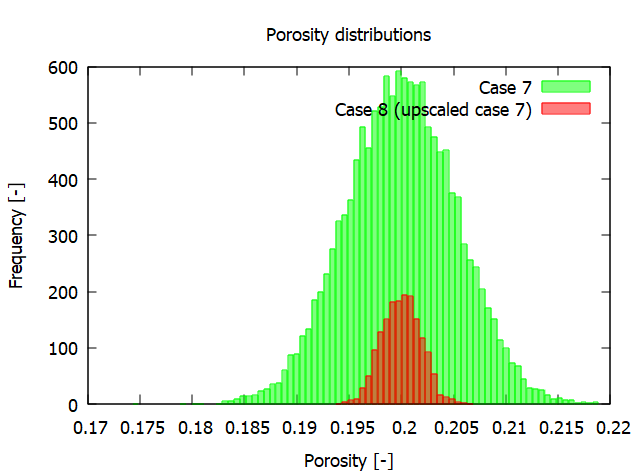
\includegraphics[width=0.8\linewidth]{Images/43}
	\caption{Porosity distribution for case 7 and its upscaled version (case 8).}
	\label{fig:43}
\end{figure}

\begin{figure}[H]
	\centering
	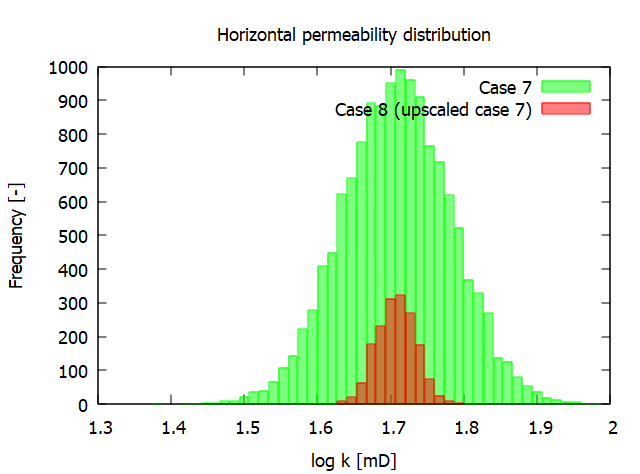
\includegraphics[width=0.8\linewidth]{Images/45}
	\caption{Horizontal permeability distribution for case 7 and its upscaled version (case 8).}
	\label{fig:45}
\end{figure}

\begin{figure}[H]
	\centering
	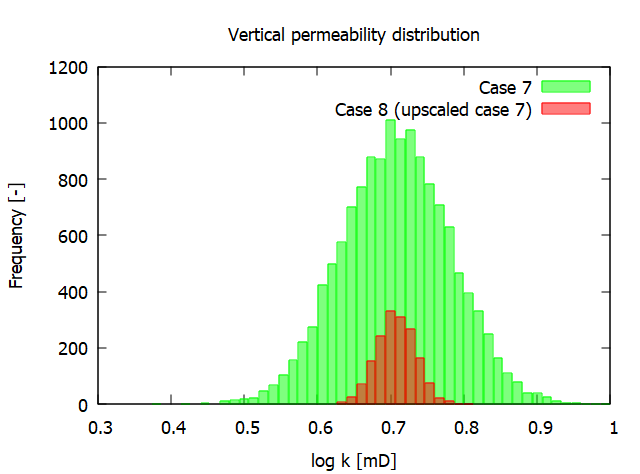
\includegraphics[width=0.8\linewidth]{Images/44}
	\caption{Vertical permeability distribution for case 7 and its upscaled version (case 8).}
	\label{fig:44}
\end{figure}

\begin{figure}[H]
	\centering
	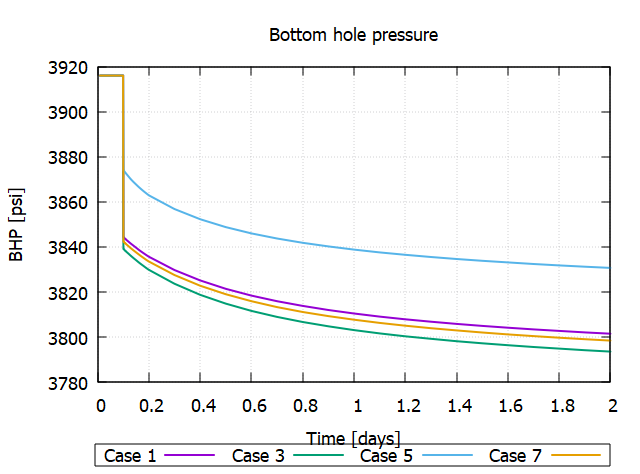
\includegraphics[width=0.8\linewidth]{Images/46}
	\caption{Bottom hole pressure for the fine models (case 1, case 3, case 5 and case 7).}
	\label{fig:46}
\end{figure}

\begin{figure}[H]
	\centering
	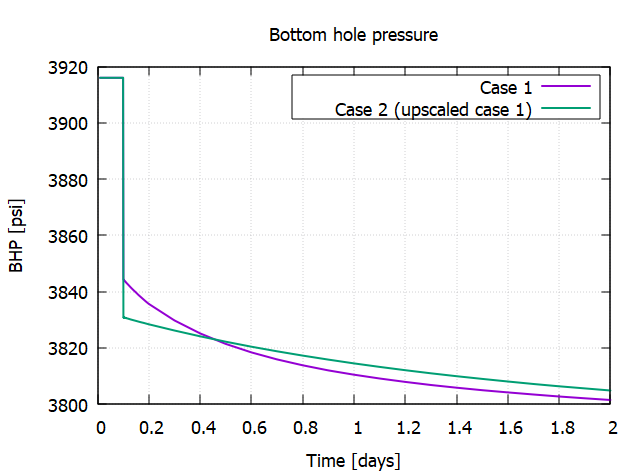
\includegraphics[width=0.8\linewidth]{Images/47}
	\caption{Bottom hole pressure for case 1 and its upscaled version, case 2.}
	\label{fig:47}
\end{figure}

\begin{figure}[H]
	\centering
	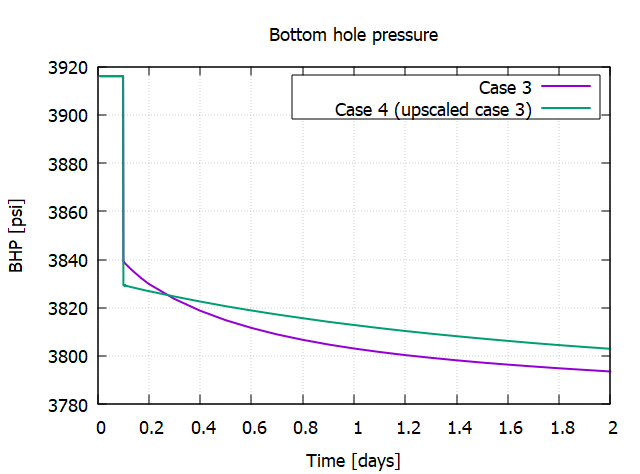
\includegraphics[width=0.8\linewidth]{Images/48}
	\caption{Bottom hole pressure for case 3 and its upscaled version, case 4.}
	\label{fig:48}
\end{figure}

Figure \ref{fig:47} shows the BHP for case 1 and case 2 (the upscaled version of case 1). One could see that the results are quite similar for each case, as expected since both cases present homogeneous porosity and permeabilities. Figure \ref{fig:48} shows similar results but for cases 3 and 4, homogeneous reservoirs. The difference between the curves is higher in those scenarios than in case 1 and 2. Nevertheless, this difference is still small, showing that the arithmetic-averaging upscaling represents the fine model with fairly good accuracy. Figures \ref{fig:49} to \ref{fig:50} display the same information for the cases 5 to 8. By looking at Figures \ref{fig:47} to \ref{fig:50}, one could see that the difference between coarse and fine models is consistently greater with higher standard deviations in the porosity and permeability distributions. 

Figure \ref{fig:51} shows the diagnostic log-log plot with the pressure drop and the Bourdet derivative for the cases 1 to 7. Case 1, 3, and 7 have very similar results. Case 5 present lower pressure drops and higher Bourdet derivatives than the other scenarios, as a consequence of its higher standard deviation. Figures \ref{fig:52} to \ref{fig:52} shows the diagnostic plot for each fine-coarse pair. Again, higher standard deviations are related to higher differences between fine and coarse curves. The Bourdet derivative is consistently lower for the coarse models in comparison with their fine pairs. Lower Bourdet derivatives are related to higher transmissibilities in the region near the wellbore. That could be one characteristic of the coarse models. 

\begin{figure}[H]
	\centering
	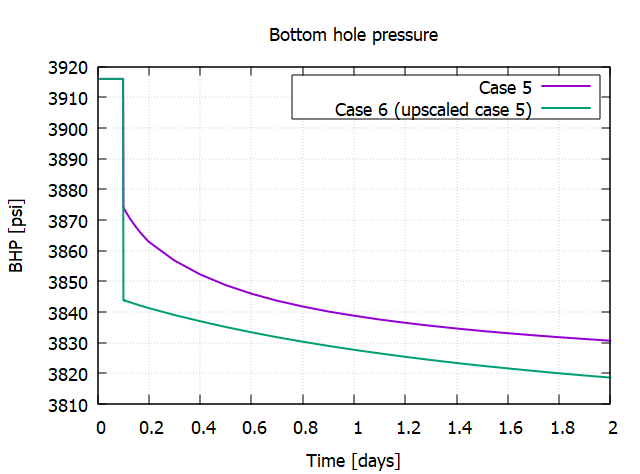
\includegraphics[width=0.8\linewidth]{Images/49}
	\caption{Bottom hole pressure for case 5 and its upscaled version, case 6.}
	\label{fig:49}
\end{figure}

\begin{figure}[H]
	\centering
	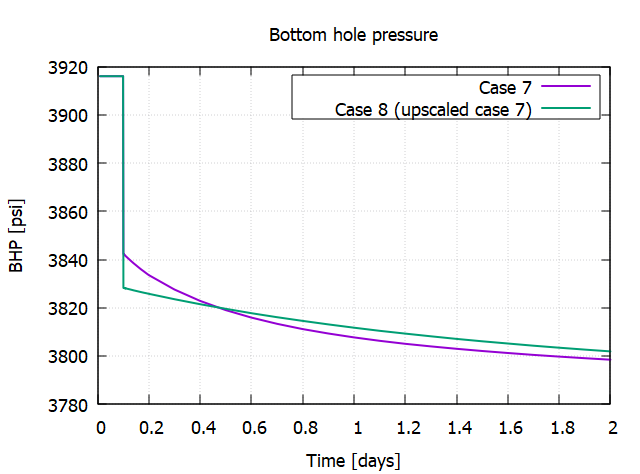
\includegraphics[width=0.8\linewidth]{Images/50}
	\caption{Bottom hole pressure for case 7 and its upscaled version, case 8.}
	\label{fig:50}
\end{figure}

\begin{figure}[H]
	\centering
	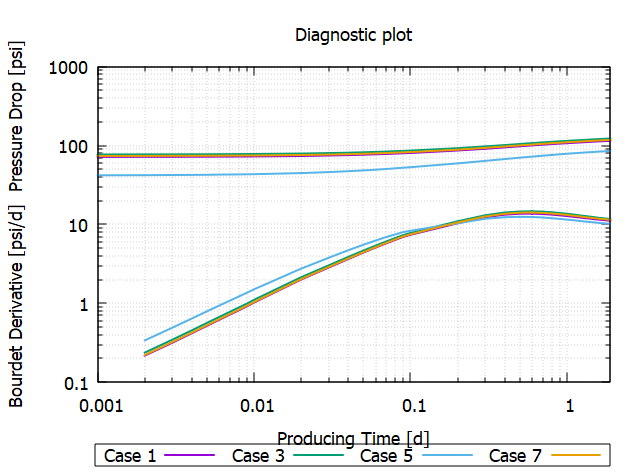
\includegraphics[width=0.8\linewidth]{Images/51}
	\caption{Pressure drop and Bourdet derivative for the fine models (case 1, case 3, case 5 and case 7).}
	\label{fig:51}
\end{figure}

\begin{figure}[H]
	\centering
	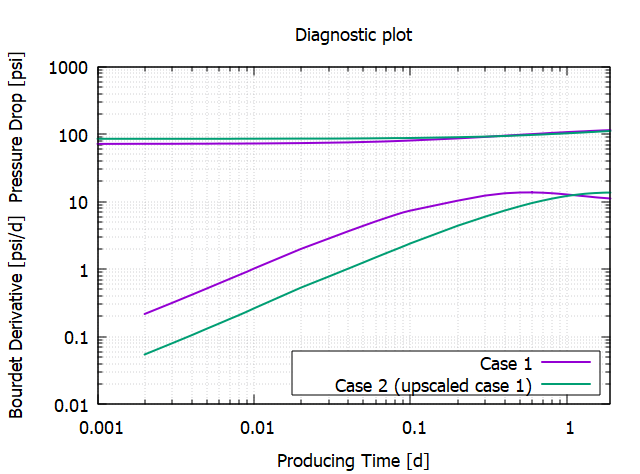
\includegraphics[width=0.8\linewidth]{Images/52}
	\caption{Pressure drop and Bourdet derivative for case 1 and its upscaled version, case 2.}
	\label{fig:52}
\end{figure}

\begin{figure}[H]
	\centering
	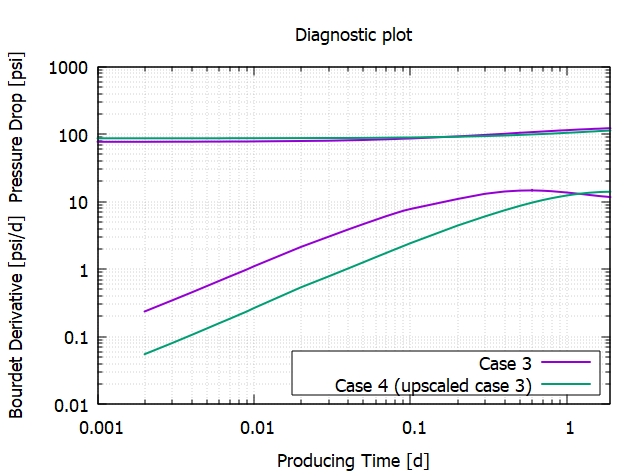
\includegraphics[width=0.8\linewidth]{Images/53}
	\caption{Pressure drop and Bourdet derivative the case 3 and its upscaled version, case 4.}
	\label{fig:53}
\end{figure}

\begin{figure}[H]
	\centering
	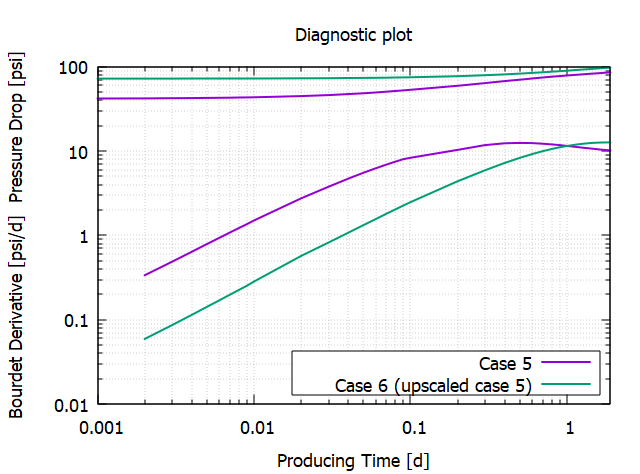
\includegraphics[width=0.8\linewidth]{Images/54}
	\caption{Pressure drop and Bourdet derivative the case 5 and its upscaled version, case 6.}
	\label{fig:54}
\end{figure}

\begin{figure}[H]
	\centering
	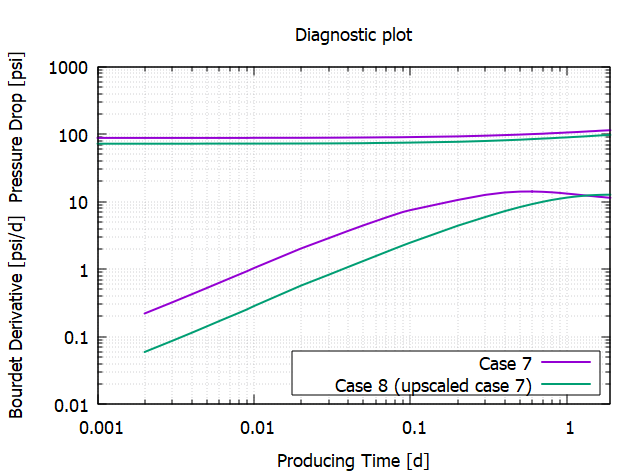
\includegraphics[width=0.8\linewidth]{Images/55}
	\caption{Pressure drop and Bourdet derivative the case 7 and its upscaled version, case 8.}
	\label{fig:55}
\end{figure}

